\documentclass{article}
\usepackage[T1]{fontenc}
\usepackage{lmodern}
\usepackage{graphicx}
\usepackage{amsmath,amssymb}
\usepackage[a4paper,margin=2cm]{geometry}
\usepackage[absolute,overlay]{textpos}
\setlength{\TPHorizModule}{1mm}
\setlength{\TPVertModule}{1mm}
\usepackage[indonesian]{babel}
\usepackage{hyperref}
\setlength{\emergencystretch}{2em}
% unit: Halaman 53

\begin{document}

% === Halaman 53 (python/native) ===

Triple DES dengan 3 kunci  (56 + 56 + 56 = 168)

E

D

X

P

K1

K2

Enkripsi

D

E

X

C

K3

K2

Dekripsi

E

K3

Y

C

D

K1

P

Y

53

% deskripsi: gambar native xref 229
\noindent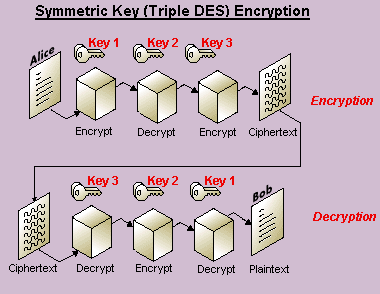
\includegraphics[width=0.85\textwidth]{../../images/python/page_053_img_01.png}

\end{document}
